\section{Auswertung}
Zu Beginn wird die lokale horizontal Komponente des Erdmagnetfeldes und die Lande-Faktoren $g_F$ der Rb-Isotope, welche in der Dampfzelle enthalten sind, ermittelt.
Dafür werden die verschiedenen Frequenzen gegen die magnetischen Feldstärken in der jeweiligen Resonanz aufgetragen. Mittels einer linearen Ausgleichsrechnung werden die $g_F$ als Steigung und die horizontal Komponente als Ordinate identifiziert.

\begin{figure}[h]
\centering
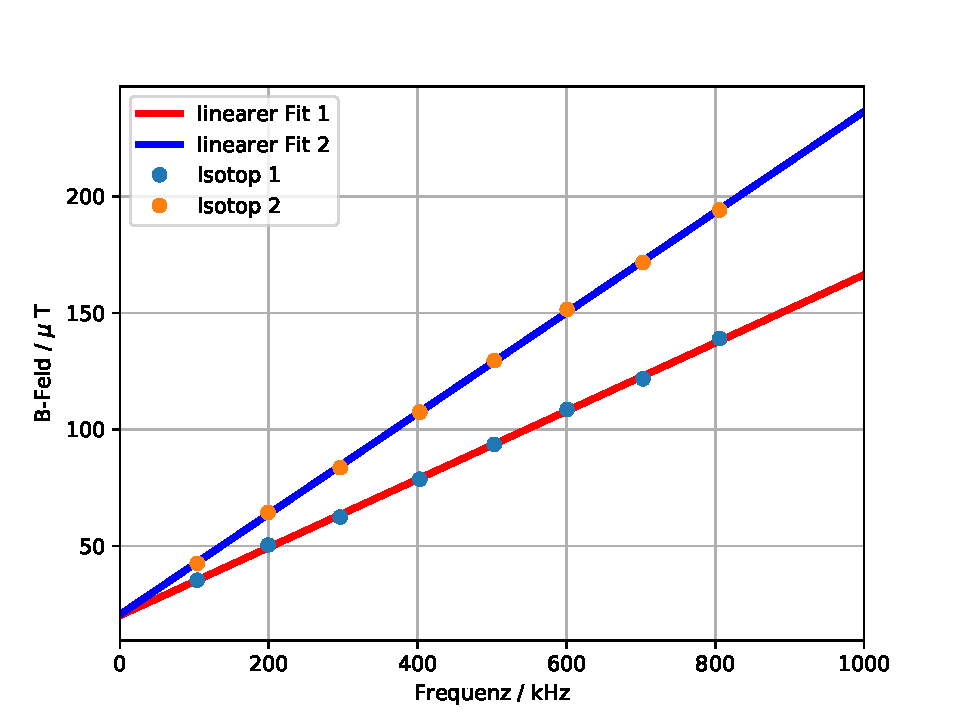
\includegraphics[scale=0.8]{./optischesPumpen/img/plotLande.pdf}
\caption{Ausgleichsrechnung zur Bestimmung der Lande Faktoren der Rb-Isotope und der lokalen horizontal Komponente des Erdmagnetfeldes}
\label{aufbau}
\end{figure}

Mit dem Ansatz
\begin{equation}
f(x) = Ax + B
\end{equation}
folgt aus der Ausgleichsrechnung folgende Werte für die Koeffizienten A und B.

\begin{table}\centering\begin{tabular}{ccc} \toprule 
\centering
\caption{Ergebnisse für die Koeffizienten A und B der Ausgleichsrechnung.}
\label{tab:isoFit}
 & A / $\mu$T/kHz  & B / $\mu$T \\ \midrule
Isotop 1 & 0.146 $\pm$ 0.001 & 20.1 $\pm$ 0.7 \\
Isotop 2 & 0.216 $\pm$ 0.001 & 20.5 $\pm$ 0.6 \\
\bottomrule
\end{tabular}
\end{table}

\newpage

Durch Koeffizientenvergleich mit gleichung 0.10 folgt für die Lande Faktoren

\begin{equation} 
g_{F1} = 0.488\pm0.005\,
label{eq:resG1}
\end{equation} 


und

\begin{equation} 
g_{F2} = 0.331\pm0.002\,
label{eq:resG2}
\end{equation} 


Außerdem lässt sich aus der Ordinate die horizontalkomponente des Erdmagnetfeldes bestimmen,
welche sich zu

\begin{equation} 
B_\text{h} = 20.3\pm0.5\,\mu\text{T}
\end{equation} 


errechnet.

In Abbildung (?) ist das Signalbild dargestellt, welches die Resonanzen zu festen
Feldstärken zeigt.

\begin{figure}[h]
\centering
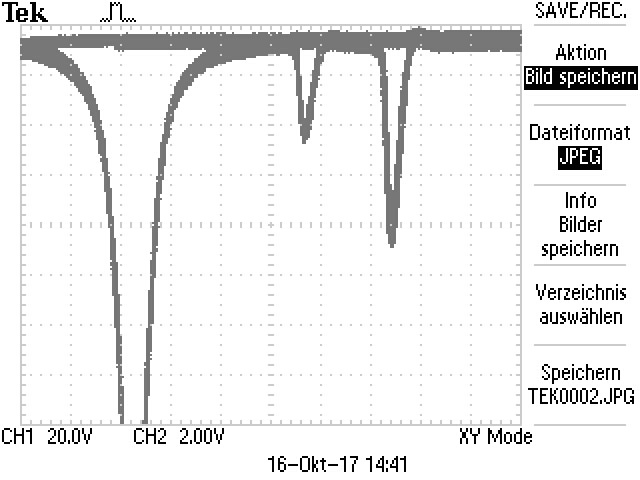
\includegraphics[scale=0.8]{./optischesPumpen/img/TEK0002.JPG}
\caption{Ausgleichsrechnung zur Bestimmung der Lande Faktoren der Rb-Isotope und der lokalen horizontal Komponente des Erdmagnetfeldes}
\label{aufbau}
\end{figure}


Aus dem Amplitudenverhältnis der Resonanzen wird das Isotopenverhältnis in der
Dampfzelle ermittelt. Dafür wird die Tiefe der Resonanzen in Pixel bestimmt.
Eine Messung der Tiefe der Resonanzen mit gimp liefert für die erste Resonanz (von links)

\begin{equation} 
h_1 = 108.0\pm1.1\,\text{px}
\end{equation} 


für die zweite Resonanz

\begin{equation} 
h_2 = 213.0\pm2.1\,\text{px}
\end{equation} 


und für das Amplitudenverhältnis

\begin{equation} 
r = 0.507\pm0.007\,
\end{equation} 


Bei der Kalkulation des Amplitudenverhältnisses wurde ein Ablesefehler von 1 Prozentpunkt
angesetzt.
